%----------------------------------------------------------------------------------------
%
% LaTeX-template for degree projects at LNU, Department of Computer Science
% Last updated by Johan Hagelbäck, Oct 2015
% Linnaeus University
%
% License: Creative Commons BY
%
%----------------------------------------------------------------------------------------

%----------------------------------------------------------------------------------------
%	Settings and configuration
%----------------------------------------------------------------------------------------

\documentclass[a4paper,12pt]{article}


\usepackage{graphicx}
%\usepackage{textcomp}
\usepackage{caption}
\usepackage{subcaption}
%\usepackage{xcolor}
\usepackage{subcaption}
\usepackage{amsmath}
\usepackage{booktabs} %for using tables in the section time plan
\usepackage{tabularx} %for auto fitting the tables
\usepackage{graphicx} %for table and booktabs
\usepackage{mathrsfs}
\usepackage{pdflscape}
\usepackage{forest}
\usepackage{pdfpages}
\usepackage{adjustbox}
\setcounter{tocdepth}{5}
\forestset{
  L1/.style={fill=green,},
  L2/.style={fill=orange,edge={orange,line width=2pt}},
  L3/.style={fill=yellow,edge={yellow,line width=2pt}},
  L4/.style={fill=pink,edge={pink,line width=2pt}},
  L5/.style={fill=pink!50,edge={pink,line width=2pt}},
}
\usepackage{xcolor}

\usepackage[T1]{fontenc}
\usepackage{times}
\usepackage[english]{babel}
\usepackage[utf8]{inputenc}
\usepackage{longtable}
%\usepackage{dtklogos}
\usepackage{wallpaper}
\usepackage[absolute]{textpos}
\usepackage[top=2cm, bottom=2.5cm, left=3.5cm, right=3.5cm]{geometry}
\usepackage{appendix}
\usepackage{lscape}
\usepackage[nottoc]{tocbibind}
\usepackage[colorlinks=true,
            linkcolor=black,
            urlcolor=blue,
            citecolor=black]{hyperref}
\usepackage{xcolor,soul}
\sethlcolor{cyan}

\setcounter{secnumdepth}{3}
\setcounter{tocdepth}{3}

\usepackage{sectsty}
\sectionfont{\fontsize{14}{15}\selectfont}
\subsectionfont{\fontsize{12}{15}\selectfont}
\subsubsectionfont{\fontsize{12}{15}\selectfont}

\usepackage{titlesec}

\titleformat{\subparagraph}[runin]
{\normalfont}
{\thesubparagraph.}{0.5em}{\underline}

\usepackage{csquotes} % Used to handle citations
\usepackage{graphicx}
\graphicspath{ {./images/} }

\renewcommand{\thetable}{\arabic{section}.\arabic{table}}  
\renewcommand{\thefigure}{\arabic{section}.\arabic{figure}} 

%----------------------------------------------------------------------------------------
%	
%----------------------------------------------------------------------------------------
\newsavebox{\mybox}
\newlength{\mydepth}
\newlength{\myheight}

\newenvironment{sidebar}%
{\begin{lrbox}{\mybox}\begin{minipage}{\textwidth}}%
{\end{minipage}\end{lrbox}%
 \settodepth{\mydepth}{\usebox{\mybox}}%
 \settoheight{\myheight}{\usebox{\mybox}}%
 \addtolength{\myheight}{\mydepth}%
 \noindent\makebox[0pt]{\hspace{-20pt}\rule[-\mydepth]{1pt}{\myheight}}%
 \usebox{\mybox}}

%----------------------------------------------------------------------------------------
%	Title section
%----------------------------------------------------------------------------------------
\newcommand\BackgroundPic{
    \put(-2,-3){
    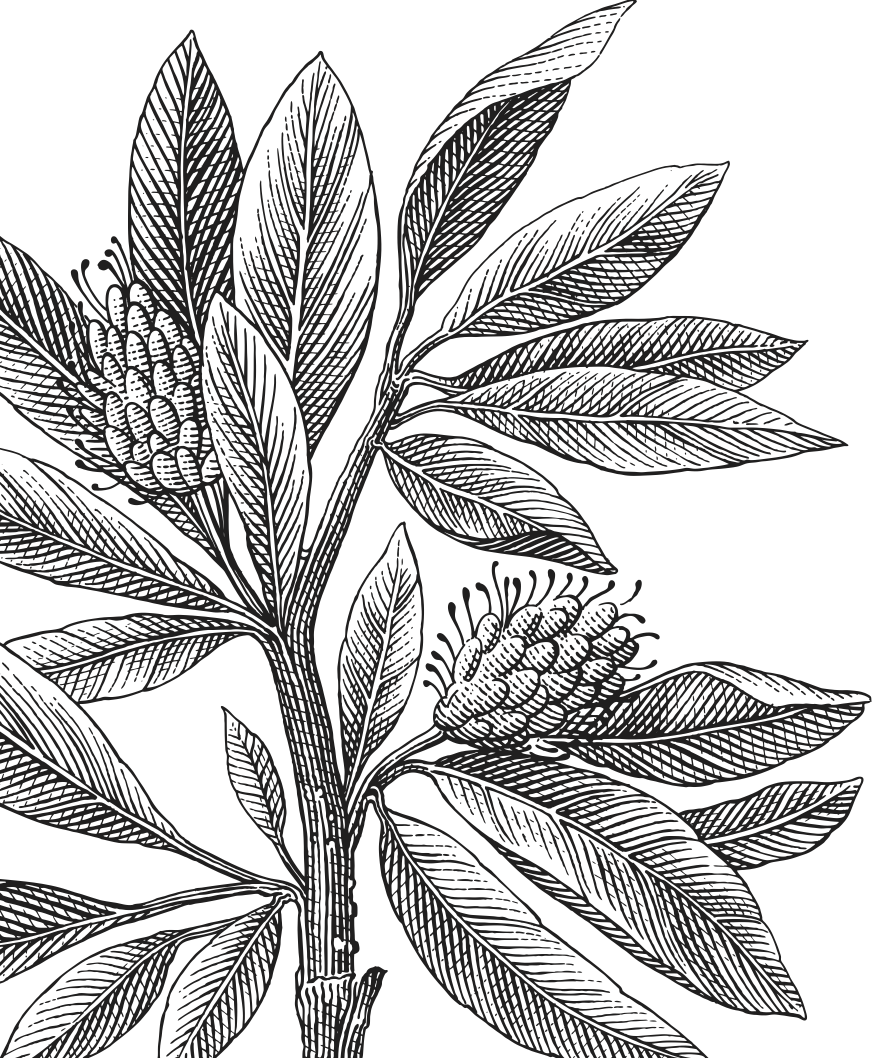
\includegraphics[keepaspectratio,scale=0.3]{img/lnu_etch.png} % Background picture
    }
}
\newcommand\BackgroundPicLogo{
    \put(30,740){
    
\includegraphics[keepaspectratio,scale=0.10]{img/logo.png} % Logo in upper left corner
    }
    \put(150,780){
    
\includegraphics[keepaspectratio]{img/text.png} % Logo in upper left corner
    }}

\title{	
\vspace{-8cm}
\begin{sidebar}
    \vspace{10cm}
    \normalfont \normalsize
    \Huge Project with Embedded System \\
    \vspace{-1.3cm}
\end{sidebar}
\vspace{3cm}
\begin{flushleft}
    \huge Title of project
\end{flushleft}
\null
\vfill
\begin{textblock}{6}(10,13)
\begin{flushright}
\begin{minipage}{\textwidth}
\begin{flushleft} \large
\emph{Authors:} ****** \textsc{*****}\\
\emph{Course Responsible:} Fredrik \textsc{Ahlgren}\\
\emph{Supervisor:} **** \textsc{*****}\\
\emph{Semester:} 23VT\\
\emph{Course code:} 2DT304
\end{flushleft}
\end{minipage}
\end{flushright}
\end{textblock}
}
\author{}
\date{} 

\begin{document}
\pagenumbering{gobble}
\newgeometry{left=5cm}
\AddToShipoutPicture*{\BackgroundPic}
\AddToShipoutPicture*{\BackgroundPicLogo}
\maketitle

\clearpage
%----------------------------------------------------------------------------------------
%	Abstract
%----------------------------------------------------------------------------------------
\selectlanguage{english}
\begin{abstract}

...



\bigskip

\textbf{Keywords:} \emph{}



\end{abstract}

%----------------------------------------------------------------------------------------
\newpage
\pagenumbering{gobble}
\tableofcontents % Table of contents
\newpage
\listoffigures
\newpage
\pagenumbering{arabic}

%----------------------------------------------------------------------------------------
%
%	Here follows the actual text contents of the report.
%
%----------------------------------------------------------------------------------------

%----------------------------------------------------------------------------------------
%    Chapters
%   Each chapter is a separate *.tex document
%   Selective compilation of chapters by setting \includeonly on the top
%----------------------------------------------------------------------------------------
\section{Introduction}


\emph{Start with some text describing the content of the chapter.}\\

\noindent This chapter will describe relevant background information for the thesis work and can be divided into different sub-chapters. Below is a suggestion, but what you use depends on what type of report you are writing and what sort of research you do. It is also possible to have the headlines in a different order if you so wish.

The introduction should pique the reader's interest in the paper and reproduce enough background information for the reader to understand the problem statement. The introduction should not be too long, then it is easy to be already here loses the reader's interest. Therefore, it shall only contain such descriptions that are relevant.

Introduction printed with a mixture of the present, past and future. For example, the present tense for what you and others think and how different things relate and the themes of the moment of writing. Imperfect of what other researchers have done and concluded. Future tense for what the investigation intends to do and what the report will describe.

One can write a first version of its introduction as the first step in the thesis. During the work, you might change this a bit. When the report is getting ready you go back and adjust the final version. It happens that the aim and questions changed during the work. It can also happens that new previous research will be added. Finally, you also want to hone some more on his introduction when you have the results, discussion and conclusion clear, so that all these parts become consistent.

\subsection{Introduction / Background}
Describe very briefly and in general terms what the project will be about. Describe maybe how you came to write about this. That one slips into a specific area may be due to initially have a query. This question is not as precise as a research question, but will perhaps lead to one. It should also explain why the topic chosen is interesting and relevant. A good way might be to pick up something from a paper, the media or the public debate to show that the topic is relevant.

Some studies involving some form of practical problem solving, perhaps on behalf of any company. Describe the practical problem area here. It may mean a brief description of the activities and mission.

In this and the next section, one can conveniently make use of a so-called "funnel" technique when writing. It involves describing the area very wide to begin with, and then taper off more and more until you get down to the report question.

\subsection{Problem definition}
Here you describe the problem that you intend to investigate. In order for work to be counted as an report you must investigate a scientific problem. In the research conducted in computer science, there is the possibility of also working with a practical problem, but this should still be linked to a scientific problem. If so, describe it then first the practical problem, and then the scientific problem. One can imagine the problem as a kind of knowledge gap that you want to make a contribution to by adding new knowledge. Examples of the problem may be that you do not know what people do on a particular issue, you do not know how something works, you do not know the reason to your problem or the lack of methods.

\subsection{Purpose and research question / hypothesis}
The purpose describes what you intend to do to investigate the problem and fill the knowledge gap. You could say that it is a kind of synthesis of the implementation. The purpose should include a specification of the type of knowledge they intend to produce. For example, descriptive knowledge, explanatory knowledge and normative knowledge (which means methods).

Depending on whether you are working deductively or inductively you should clarify its purpose in one or more hypotheses or questions. A hypothesis is an assumption about how something relates, that it intends to investigate whether it is true or not. For example, to assume that all systems development companies follow a system development method, which it intends to investigate whether it is true or not. The hypothesis is always based in theory or prior research. We must therefore know something before we can formulate a hypothesis. This means working deductively.

If you do not know something (not you personally, but the scientific community), you get instead work inductively. Then we formulate one or more research questions. These questions must be answered by the inquiry to make. Conclusion of the report is thus a direct response to the research questions. A research question can be for example; "What systems development methodologies are used in systems development company?". The research questions are clearer specification of the initial puzzlement as they might have.

\subsection{Scope / Limitation}
Here you describe what you do not intend to do in your investigation. It is important not to confuse this with the selection describing the methodology chapter. Therefore, you should not write that you will interview the X and Y, but not Z. Your limitations should be relevant to the purpose in question. Therefore, they should not specify that they opted out to study the rest of the world. Some limitations make you maybe from the beginning, while others naturally to come during the work. Explain also why this will not be studied. Time is a common reason why aspects must be deselected. Note, however, to describe it in a professional manner and you shall not make excuses.

\subsection{Target group}
This section is not mandatory. However, this can be good both when writing and later on for the reader. Here you describe for whom you intend to give a knowledge contribution to. If I as a reader is mentioned in the target group, I know of course that this paper should be of interest for me to read.

If you plan to make a practical contribution to a specific group of persons or activities you describe it here. It is not enough to mention this target group to classify this report as a scientific paper. You must target it to a more general and scientific audience. To describe this audience here and constantly thinking about writing for them is a great way to ensure that it becomes a scientific paper writing.

It is not enough to have the supervisor and examiner as that audience. If you can not come to a broader audience, perhaps the  chosen topic is not interesting, relevant and innovative enough.

\subsection{Outline}
For the reader it can be helpful to have a description of the various coming chapters and sections of the report and how these relate to each other. Here we can also provide reading instructions for specific groups of readers if you so wish.
\section{Related Work }
\emph{Start with some text describing the content of the chapter.}\\


\begin{itemize}
    \item  Has anyone done a project like this before? 
    \item  How does your project compare to existing similar projects?
\end{itemize}  
 
\section{Hardware}
\emph{Start with some text describing the content of the chapter.}\\


\begin{itemize}
    \item Embedded Board Description: Describe the hardware, CPU (architecture, type, speed), RAM, and I/O.  Also describe the operating system or other software (kernel version, etc.)
    \item Input device description: Describe the device you are interfacing with, how you access it in software and document the protocol you use to communicate with it
    \item Output Device description: same as for the input device.
    \item Links to any datasheets for hardware you used, as well as schematics for any circuits you designed yourself
    \item Power Consumption: Explain any energy or power concerns with your application, and how you could optimize it to use less power.

        
\end{itemize}

\section{Software}
\emph{Start with some text describing the content of the chapter.}\\


\begin{itemize}
    \item Programming Language:  Which one did you use? Why? Briefly explain the tradeoffs between the language you chose and doing the same in assembly language.
    \item Real-Time: Does your device have real-time constraints? What would happen if your code encountered an unexpectedly large delay?
    \item Security: Describe any computer security issues there might be with your device (can it be exploited?) If you say there are no security issues, make sure you explain why
    \item If you use code not written by your group (code found online, libraries, etc) explain what the extra code does, and how your code interfaces with it. Explain how much of the code is original to your group.

\end{itemize}

\section{Results and Discussion}
\emph{Start with some text describing the content of the chapter.}\\

\noindent What you describe in this chapter depends very much on what type of study you have done. In this chapter you describe your analysis. How this is done depends on the type of analysis to do. In a quantitative study, the results of various statistical analyzes and comparisons of different issues are done here. It is also possible to aggregate the result and analysis chapter to one chapter. In a qualitative study, one can demonstrate the patterns that have been  recognized based on the material. It may also be in order to apply a theoretical model on the empirical material, or otherwise make connections between theory and empirical data to describe, explain or point out the connection. The analysis shall be more clean and maintained without discussion. In qualitative studies, it is common to add the analysis and discussion 

\section{Conclusion}
\emph{Start with some text describing the content of the chapter.}\\

\begin{itemize}
    \item If you worked in a group: List who worked on what part
    \item Challenges: List any challenges you had, and if things didn’t work, explain why
    \item Future  Work: List any improvements you might make if you had more time and resources to work on the project.
    
\end{itemize}













\newpage
\hypersetup{urlcolor=black}
\bibliographystyle{IEEEtran}
\bibliography{referenser}
\newpage
\clearpage
\setcounter{page}{1} % Starting on page 1 for attachments
\appendix

\chapter{Appendix 1} % Append '*' to skip from table of contents (TOC)
It may often be appropriate to put details in the appendices, as they briefly has been explained in the main report and there been given a reference to details via see Appendix X.

\begin{subappendices}

\section{Appendix 1.1 }
The source code (this can be submitted as a separate file, does not have to be included in the report).

\section{Appendix 1.2}
Make a short website or  YouTube video describing your project and share the link here.
\end{subappendices}


\end{document}
